\textbf{Modify program ssq2 to account for a finite queue capacity.}\\\\

\noindent \textbf{(a) For the queue capacities 1,2,3,4,5, and 6, construct a table of the estimated steady-state probability of rejection.}\\\\

\begin{table}[h]
\centering
\begin{tabular}{l|lll}
Uniform(1.0, 2.0) & 123456 & 246810 & 97531 \\
\hline\\
Rejection Q = 1   & 18.53  & 18.45  & 18.19 \\
Rejection Q = 2   & 8.98   & 9.05   & 8.78  \\
Rejection Q = 3   & 4.77   & 4.76   & 4.55  \\
Rejection Q = 4   & 2.65   & 2.61   & 2.51  \\
Rejection Q = 5   & 1.45   & 1.52   & 1.35  \\
Rejection Q = 6   & 0.83   & 0.85   & 0.74 
\end{tabular}
\end{table}

\noindent \textbf{(b) Also, construct a similar table if the service-time distribution is changed to be $Uniform(1.0, 3.0)$.}\\\\

\begin{table}[h]
\centering
\begin{tabular}{l|lll}
Uniform(1.0, 3.0) & 123456 & 246810 & 97531 \\
\hline\\
Rejection Q = 1   & 27.66  & 27.58  & 27.24 \\
Rejection Q = 2   & 18.45   & 18.30   & 18.11  \\
Rejection Q = 3   & 13.82   & 13.69   & 13.41  \\
Rejection Q = 4   & 10.93   & 10.77   & 10.55  \\
Rejection Q = 5   & 9.05   & 8.86   & 8.60  \\
Rejection Q = 6   & 7.74   &   7.55 & 7.43 
\end{tabular}
\end{table}

\noindent \textbf{(c) Comment on how the probability of rejection depends on the service process.}\\\\

\noindent The probability of rejection increases when the service time increases. This makes sense, as a higher service time allows the queue to build up, particularly when the interarrival rate is faster than the service time.\\\\

\noindent \textbf{(d) How did you convince yourself these tables are correct?}\\\\
This makes sense, as the increased service time increases the rejection rate. Additionally, a longer queue makes the rejection rate decrease, as the service node can handle multiple jobs arriving in a short period of time given that the queue has space. \\\\
\begin{center}
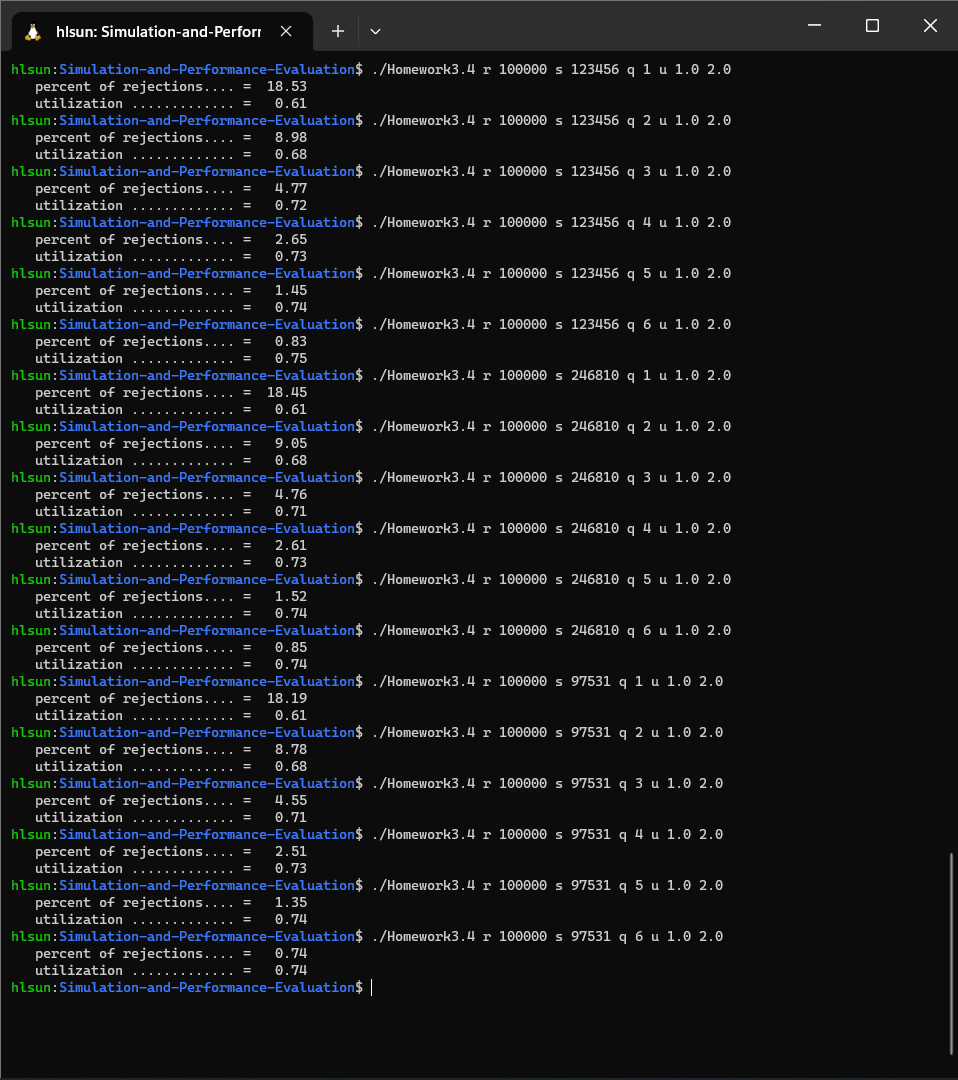
\includegraphics[scale=0.75]{Sections/Q4/H3_4_A.png}\\
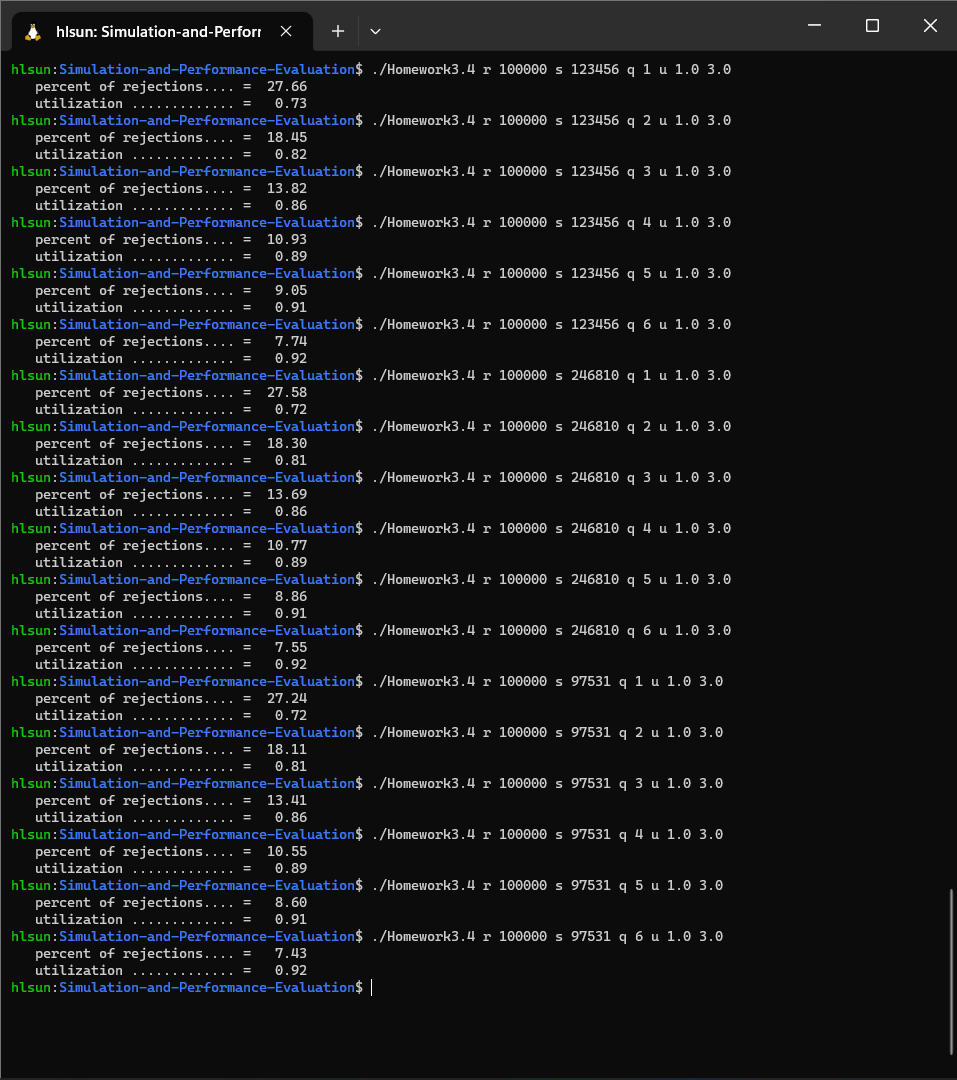
\includegraphics[scale=0.75]{Sections/Q4/H3_4_B.png}\\
\end{center}

\begin{lstlisting}[style=CStyle]
/**
 * Modified by Harrison Sun
 * sun.har@northeastern.edu
 * February 11, 2023
 */

 /* -------------------------------------------------------------------------
  * This program is a next-event simulation of a single-server FIFO service
  * node using Exponentially distributed interarrival times and Uniformly
  * distributed service times (i.e., a M/U/1 queue).  The service node is
  * assumed to be initially idle, no arrivals are permitted after the
  * terminal time STOP, and the service node is then purged by processing any
  * remaining jobs in the service node.
  *
  * Name            : ssq3.c  (Single Server Queue, version 3)
  * Author          : Steve Park & Dave Geyer
  * Language        : ANSI C
  * Latest Revision : 10-19-98
  * -------------------------------------------------------------------------
  */

#include <cstdlib>
#include <cstring>
#include <stdio.h>
#include <exception>
#include <iostream>
#include <math.h> 
#include <string>
#include "c_lib/rvgs.h"
#include "c_lib/rngs.h"

#define START         0.0              /* initial time                   */
#define STOP      20000.0              /* terminal (close the door) time */
//#define INFINITY   (10000.0 * STOP)  /* must be much larger than STOP  */
#define MAXQUEUE     6                 /* max. # of jobs in queue        */


double Min(double a, double c)
/* ------------------------------
 * return the smaller of a, b
 * ------------------------------
 */
{
    if (a < c)
        return (a);
    else
        return (c);
}

double GetArrival()
/* ---------------------------------------------
 * generate the next arrival time
 * ---------------------------------------------
 */
{
    static double arrival = START;

    SelectStream(0);
    arrival += Exponential(2.0);
    return (arrival);
}


double GetService(double lb, double ub)
/* --------------------------------------------
 * generate the next service time with rate 2/3
 * --------------------------------------------
 */
{
    SelectStream(1);
    return (Uniform(lb, ub));
}

/**
* bool checkArg()
*
* @param char* input - the input string literal from the console
* @return bool - true if the input is a number, false otherwise
*
* This function determines whether the argument is a number.
*/

bool checkArg(char* input)
{
    try
    {
        if (strlen(input) > 9)
        {
            throw std::logic_error("Number is too large.");
        }

        for (int i = 0; i < strlen(input); ++i)
        {

            if (std::isdigit(input[i]) || (input[i] == '.')) continue;
            else
            {
                std::string errorMessage;
                errorMessage.append((std::string)input);
                errorMessage.append(" is not a number.");
                throw std::logic_error(errorMessage);
            }
        }
        return 1;
    }

    catch (const std::logic_error& error)
    {
        std::cerr << error.what() << std::endl;
        return 0;
    }
}

int main(int argc, char* argv[])
{
    struct {
        double arrival;                 /* next arrival time                                */
        double completion;              /* next completion time                             */
        double current;                 /* current time                                     */
        double next;                    /* next (most imminent) event time                  */
        double last;                    /* last arrival time                                */
    } t;
    struct {
        double node;                    /* time integrated number in the node               */
        double queue;                   /* time integrated number in the queue              */
        double service;                 /* time integrated number in service                */
    } area = { 0.0, 0.0, 0.0 };
    long index{};                       /* used to count departed jobs                      */
	long reject{};                      /* number of jobs rejected because of full queue    */
    long number{};                      /* number in the node                               */
    double endtime{};
    int queuesize{};
    double lowerBound{};
    double upperBound{};
    // Set the seed
    for (int i = 0; i < argc; ++i)
    {
        if (*argv[i] == 's' && checkArg(argv[i + 1]))
        {
            PlantSeeds(std::stol(argv[i + 1]));
            break;
        }
        else
        {
            PlantSeeds(123456789);
        }
    }

    // Set the number of runs
    for (int i = 0; i < argc; ++i)
    {
        if (*argv[i] == 'r' && checkArg(argv[i + 1]))
        {
            endtime = std::stol(argv[i + 1]);
            break;
        }
        else
        {
            endtime = STOP;
        }
    }

    // Set the queue size
    for (int i = 0; i < argc; ++i)
    {
        if (*argv[i] == 'q' && checkArg(argv[i + 1]))
        {
            queuesize = std::stol(argv[i + 1]);
            break;
        }
        else
        {
            queuesize = MAXQUEUE;
        }
    }

    // Set the bounds for uniform distribution (service time)
    for (int i = 0; i < argc; ++i)
    {
        if (*argv[i] == 'u' && checkArg(argv[i + 1]) && checkArg(argv[i + 1]))
        {
			lowerBound = std::stol(argv[i + 1]);
			upperBound = std::stol(argv[i + 2]);
            break;
        }
        else
        {
			lowerBound = 1.0;
			upperBound = 2.0;
        }
    }
    t.current = START;           /* set the clock                         */
    t.arrival = GetArrival();    /* schedule the first arrival            */
    t.completion = INFINITY;        /* the first event can't be a completion */

    while ((t.arrival < endtime) || (number > 0)) {
        t.next = Min(t.arrival, t.completion);          /* next event time   */
        if (number > 0) {                               /* update integrals  */
            area.node += (t.next - t.current) * number;
            area.queue += (t.next - t.current) * (number - 1);
            area.service += (t.next - t.current);
        }
        t.current = t.next;                         /* advance the clock */

        if (t.current == t.arrival) {               /* process an arrival */
            if (number < queuesize)
            {
                number++;
                t.arrival = GetArrival();
                if (t.arrival > endtime) {
                    t.last = t.current;
                    t.arrival = INFINITY;
                }
                if (number == 1)
                    t.completion = t.current + GetService(lowerBound, upperBound);
            }
            else
            {
				reject++;
                t.arrival = GetArrival();
                if (t.arrival > endtime) {
                    t.last = t.current;
                    t.arrival = INFINITY;
                }
                if (number == 1)
                    t.completion = t.current + GetService(lowerBound, upperBound);
            }
        }

        else {                                        /* process a completion */
            index++;
            number--;
            if (number > 0)
                t.completion = t.current + GetService(lowerBound, upperBound);
            else
                t.completion = INFINITY;
        }
    }

    printf("\nfor %ld jobs\n", index);
    printf("   average interarrival time = %6.2f\n", t.last / index);
    printf("   average wait ............ = %6.2f\n", area.node / index);
    printf("   average delay ........... = %6.2f\n", area.queue / index);
    printf("   average service time .... = %6.2f\n", area.service / index);
    printf("   average # in the node ... = %6.2f\n", area.node / t.current);
    printf("   average # in the queue .. = %6.2f\n", area.queue / t.current);
	printf("   number of rejections..... = %6.2ld\n", reject);
	printf("   percent of rejections.... = %6.2f\n", ((double)reject / (index+reject)) * 100);
    printf("   utilization ............. = %6.2f\n", area.service / t.current);

    return (0);
}
\end{lstlisting}